\documentclass[10pt, letterpaper, oneside]{article}
\usepackage[hmargin={0.5in,0.5in},vmargin={2.58in,1.2in},
            showframe,
            %headheight=1.2in,
            %headsep=15pt,
            verbose]{geometry}
\usepackage[utf8]{inputenc}
\usepackage[T1]{fontenc}
\usepackage[english]{babel}
%\usepackage[onlytext]{MinionPro}
\usepackage[normalem]{ulem}
\usepackage[inline]{enumitem}
\usepackage{amssymb}
\usepackage{adjustbox}
\usepackage{graphicx}
\usepackage[yyyymmdd,hhmmss]{datetime}
\usepackage{eso-pic}
\usepackage{longtable}

\graphicspath{{./src/}}

\usepackage{fontspec}
\setmainfont{Helvetica Neue}
%\setmainfont{Gill Sans}
%\setmainfont{PT Sans}

\usepackage{microtype}
\usepackage[colorlinks,citecolor=black,urlcolor=blue,breaklinks,unicode]{hyperref}

\setlength{\parskip}{1.5ex} % 1ex plus 0.5ex minus 0.2ex}
\setlength{\parindent}{0pt}

\title{}
\author{}

\newcommand\BackgroundPic{
    \put(0,0){
    \parbox[b][\paperheight]{\paperwidth}{%
    \vfill
    \centering
    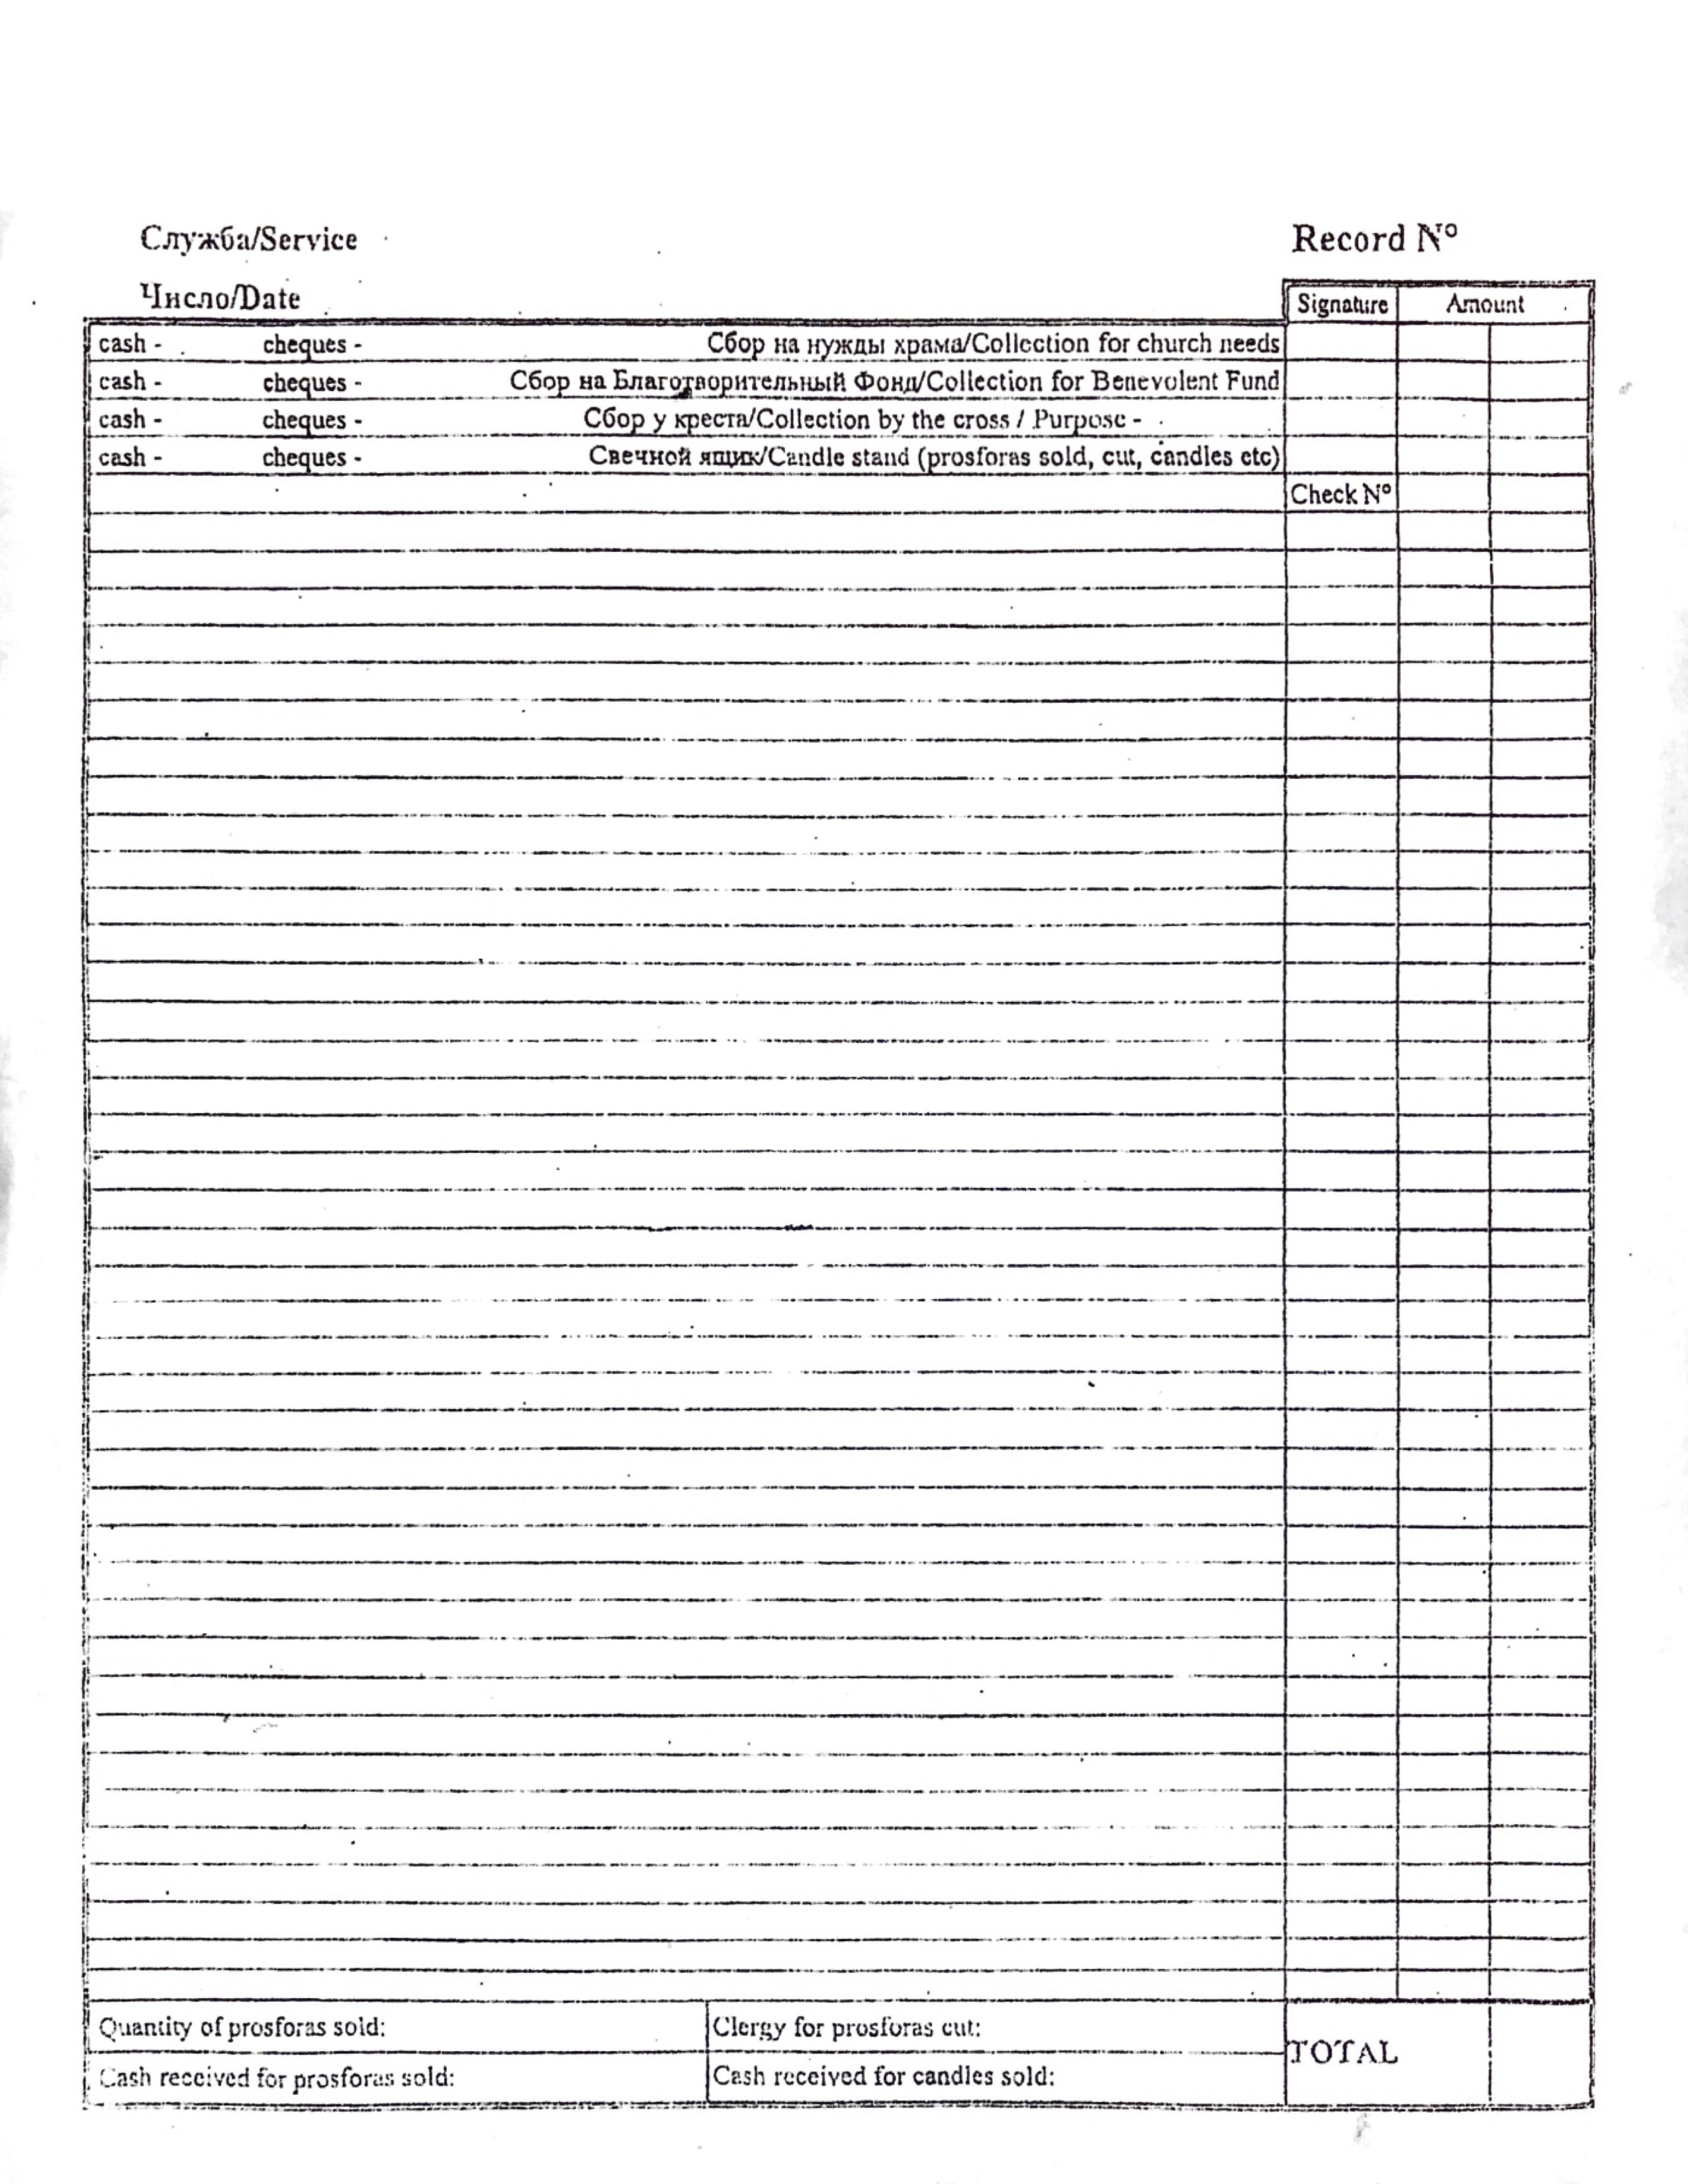
\includegraphics[width=\paperwidth,height=\paperheight]{poop_sheet_bkg.jpg}
    \vfill
    }}}

\renewcommand{\baselinestretch}{1.14}

\newcommand{\rpt}{%
        \raisebox{.2ex}{:}%
        \raisebox{-.4ex}{\rule{.1ex}{2.5ex}\,\rule{.3ex}{2.5ex}}}
\newcommand{\revrpt}{%
        \raisebox{-.4ex}{\rule{.3ex}{2.5ex}\,\rule{.1ex}{2.5ex}}%
        \raisebox{.2ex}{:}}

\begin{document}
\AddToShipoutPicture{\BackgroundPic}
\selectlanguage{english}

\BLOCK{set ns = namespace(payor = "",method="",identifier="",charge="")}
\begin{longtable}[l]{l l l l l}
\BLOCK{for row in data}
    \BLOCK{set payor = row["Payor"]}
    \BLOCK{set method = row["Method"]}
    \BLOCK{set charge = row["Charge"]}
    \BLOCK{if charge != ns.charge}
        \BLOCK{set ns.charge = charge}
        \\
        \\
    \BLOCK{endif}
    \parbox{2.75in}{
        \BLOCK{if payor != ns.payor}
            \BLOCK{set ns.payor = payor}
            \VAR{payor}
        \BLOCK{else}
            ~~~~~ \textquotedbl ~~~~~ \textquotedbl ~~~~~ \textquotedbl
        \BLOCK{endif}
    } &
    \parbox{2.4in}{\VAR{row["Purpose"]}} & 
    \parbox{0.35in}{\raggedleft 
        \BLOCK{if method == ""}
            ~
        \BLOCK{else}
            \VAR{method}
        \BLOCK{endif}
    } & 
    \parbox{0.4in}{\raggedleft \VAR{row["Identifier"]}} & 
    \parbox{0.3in}{\raggedleft \VAR{row["Amount"]}} \\
\BLOCK{endfor}
\end{longtable}

\end{document}

